\documentclass[superscriptaddress,onecolumn,pre]{revtex4}

\usepackage{ifthen}
\newboolean{pnas}
\setboolean{pnas}{false}

\usepackage{amsmath}
\usepackage{amsfonts}
\usepackage{amssymb}
\usepackage{mathtools}
\usepackage{graphicx}
\usepackage[T1]{fontenc}
\usepackage[utf8]{inputenc}
\graphicspath{{images/}}
\usepackage{color}
\usepackage[pdfstartview=FitH,
            breaklinks=true,
            bookmarksopen=false,
            bookmarksnumbered=true,
            colorlinks=true,
            linkcolor=black,
            citecolor=black,
            urlcolor=black,
            pdftitle={Peptidome},
            pdfauthor={Andreas Mayer},
            pdfsubject={}
            ]{hyperref}
\newcommand{\B}{\boldsymbol}
\newcommand{\ud}{\mathrm{d}}
\newcommand{\<}{\langle}
\renewcommand{\>}{\rangle}

\def\(({\left(}
\def\)){\right)}                       
\def\[[{\left[}
\def\]]{\right]}

\newcommand{\AM}[1]{{\color{blue}#1}}

\begin{document}

\title{Figures}
%\author{Andreas Mayer}
%\author{Quentin Marcou}
%\author{Warren James}
%\author{Christopher Russo}
%\author{William Bialek*}
%\author{Benjamin D Greenbaum*}
\date{\today}

\maketitle

\begin{figure}
    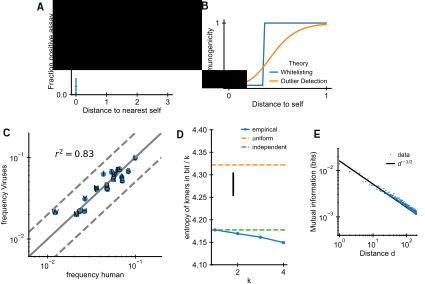
\includegraphics{figure1}
    \caption{Testing prior models of self/non-self peptide discrimination}
\end{figure}

\begin{figure}
    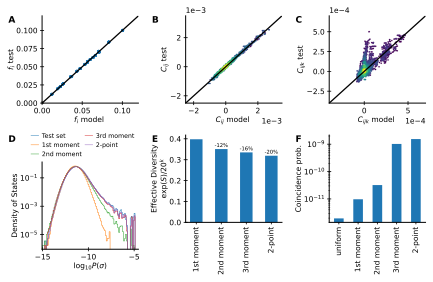
\includegraphics{figure2}
    \caption{Maximum entropy model predicts peptide statistics}
\end{figure}


\begin{figure}
    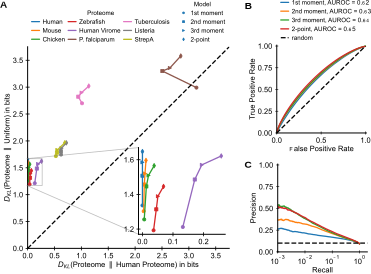
\includegraphics{figure3}
    \caption{Divergence between peptides from different proteomes}
\end{figure}

\begin{figure}
    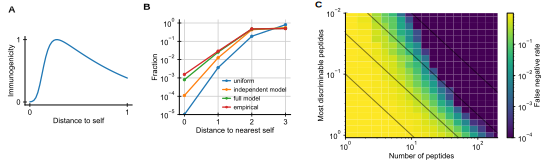
\includegraphics{figure4}
    \caption{A theory of immune discrimination in the light of shared proteome biases}
\end{figure}

\begin{figure}
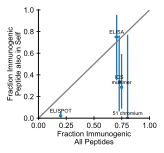
\includegraphics{figureS1}
\caption{Differences between assays measuring immunogenicity}
\end{figure}

\end{document}
